Trong quá trình xây dựng hệ thống, cần có trao đổi giữa người thiết kế hệ thống và chuyên gia miền. Tuy nhiên, nhóm kinh doanh sử dụng ngôn ngữ kinh doanh và nhóm công nghệ có xu hướng sử dụng các thuật ngữ kỹ thuật trong giao tiếp của họ. Người phát triển phần mềm tập trung vào lớp, phương thức, thuật toán, \dots Chuyên gia miền thường sử dụng ngôn ngữ chuyên ngành của họ. Sự khác biệt về ngôn ngữ giữa các thành viên có thể dẫn đến những thách thức về giao tiếp. Ngoài ra, trong các lĩnh vực kinh doanh khác nhau, một thuật ngữ có thể được sử dụng trong nhiều miền, cùng với ý nghĩa khác nhau gây ra sự nhầm lẫn và hiểu sai cho các người phát triển phần mềm cũng như các chuyên gia miền.

Thiết kế hướng miền đề xuất sử dụng ngôn ngữ chung để giải quyết những thách thức ngôn ngữ. \emph{Ngôn ngữ chung (Ubiquitous Language)} là một ngôn ngữ được cấu trúc xung quanh mô hình miền và được tất cả các thành viên trong nhóm sử dụng cho mọi hoạt động của nhóm với phần mềm. Ngôn ngữ chung được xác định bởi các từ vựng và có định nghĩa rõ ràng về ngữ cảnh sử dụng từ vựng.

\subsubsection{Một số đặc điểm của ngôn ngữ chung}

\begin{itemize}

\item Ngôn ngữ chung được sử dụng bởi cả chuyên gia miền và chuyên gia công nghệ.

\item Có nhiều ngôn ngữ chung trong một tổ chức được mỗi nhóm tạo và quản lý độc lập.

\item Việc tạo ra ngôn ngữ chung là một quá trình liên tục, phát triển theo thời gian qua sự cộng tác giữa chuyên gia miền và chuyên gia công nghệ.

\item Các thành viên phải sử dụng ngôn ngữ chung cho các công việc và trong hệ thống.

\end{itemize}

\begin{figure}[H]

\centering

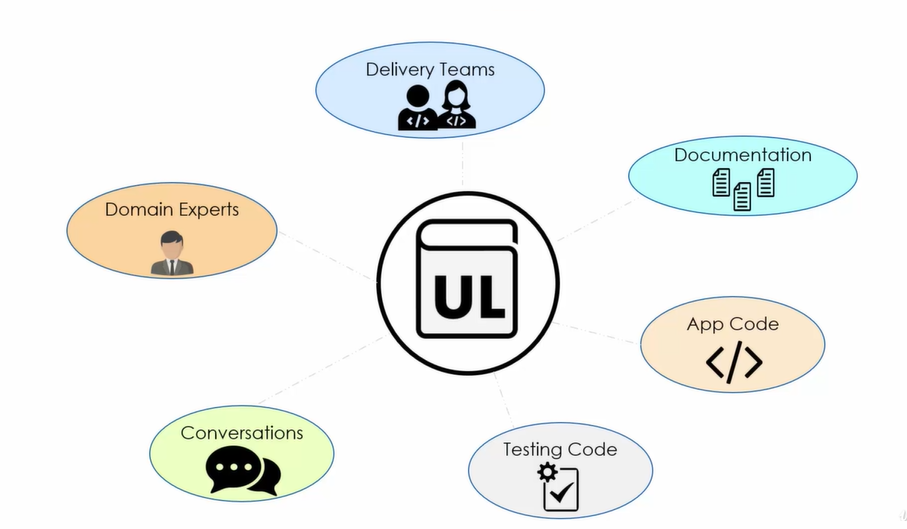
\includegraphics[scale = 0.6]{pictures/_ngon_ngu_chung_duoc_su_dung_trong_toan_bo_he_thong/main.png}

\caption{Ngôn ngữ chung được sử dụng trong toàn bộ hệ thống}

\end{figure}

\begin{example} Trong đồ án này, em đã sử dụng ngôn ngữ chung trong toàn bộ hệ thống của mình từ yêu cầu nghiệp vụ, mã nguồn, kiểm thử, \dots \end{example}